\documentclass{IEEEtran}

\usepackage{graphicx}
\usepackage{hyperref}

\title{An evaluation of various 3D/3D multimodal medical image registration methods}
\author{Sihan Li, Tsinghua University}

\begin{document}
  \maketitle

  \begin{abstract}
    This paper aims to compare different 3D/3D multimodal medical image registration methods. Methodologies using different similarity measures are implemented. Dataset from Retrospective Image Registration Evaluation Project (RIRE) is used to evaluate various implementations. The accuracy of each implementation is presented.

  \end{abstract}

  \section{Introduction}
    Many toolboxes have been developed to achieve the goal. MATLAB Image Processing Toolbox offers an automatic intensity-based routine to register 2D or 3D images. It is rather easy to use, but it only support few metrics or optimizers. It is also not possible to add new metrics or optimizers without re-implementing almost everything, as only binaries of internal implementations are given. Medical Image Registration Toolbox (MIRT) \cite{myronenko2007lv, myronenko2009adaptive, myronenko2009image, myronenko2009maximum, myronenko2010intensity} contains a set of MATLAB functions to do registration. But it is not updated often, and it can only handle non-rigid registration. Elastix \cite{klein2010elastix} is a popular software package for image registration implemented in C++ based on Insight Toolkit (ITK). It is an open source project and is maintained by many developers. It also very customizable, both by parameters adjustment or implementing new modules. Other options include A Flexible Image Registration Toolbox (FLIRT) \cite{papenberg2007fast} etc.

    Retrospective Image Registration Evaluation Project (RIRE) is a project designed to compare different registration techniques. It contains a set of CT, PET and MR images. Each MR-CT images pair and MR-PET images pair has been corrected using frames and markers, so the results of different registration methods can be compared with the ``true'' registration results. We are using RIRE to measure the performance of different registration methodologies.

    Because RIRE expects a rigid transformation, we will only implement and compare area-based metrics discussed in our last report. To be precise, we will use MATLAB Image Processing Toolbox and elastix to implement a set of methodologies. Different similarity metrics will be applied and compared, including mean squared difference (MSD), normalized correlation coefficient (NCC), mutual information (MI) and normalized mutual information (NMI).

  \section{Methods}

  For the implementations using MATLAB Image Processing Toolbox, we use \texttt{OnePlusOneEvolutionary} optimizers, as well as \texttt{MeanSquares} and \texttt{MattesMutualInformation} metrics. For the implementations using elastix, the default parameter set is used except \texttt{Metric} field, where different similarity metrics (\texttt{AdvancedMeanSquares}, \texttt{AdvancedNormalizedCorrelation}, \texttt{AdvancedMattesMutualInformation} and \texttt{NormalizedMutualInformation}) are used in corresponding implementation. The source code is available at \url{https://github.com/ThomasLee969/stanford-project}.

  \section{Results}

  We adopt the methodologies using in \cite{pluim2004f} to evaluate the accuracy of each implementation. The 0.5 and 0.9 quantile errors over all CT-MR and PET-MR pairs of patient 001 to 009 have been calculated. The results can be seen in Figure~\ref{fig:CT-MR_bars} and Figure~\ref{fig:PET-MR_bars}.

  \begin{figure}[htbp]
    \centering
    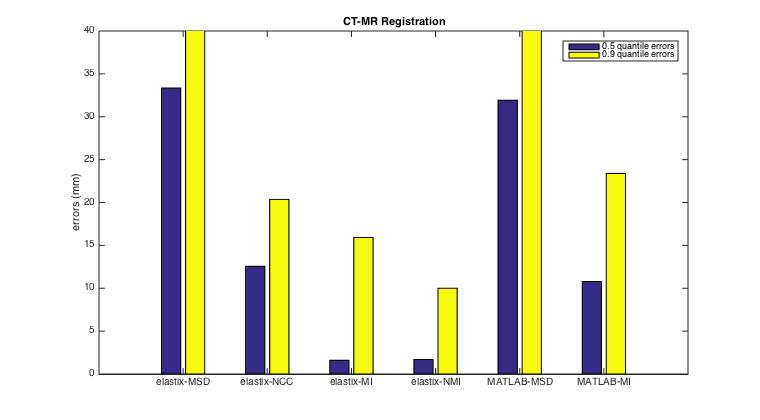
\includegraphics[width=0.5\textwidth]{CT-MR_bars.png}
    \caption{Quantile errors for CT to MR registration. Errors larger than 40 mm have been cut off.}
    \label{fig:CT-MR_bars}
  \end{figure}

  \begin{figure}[htbp]
    \centering
    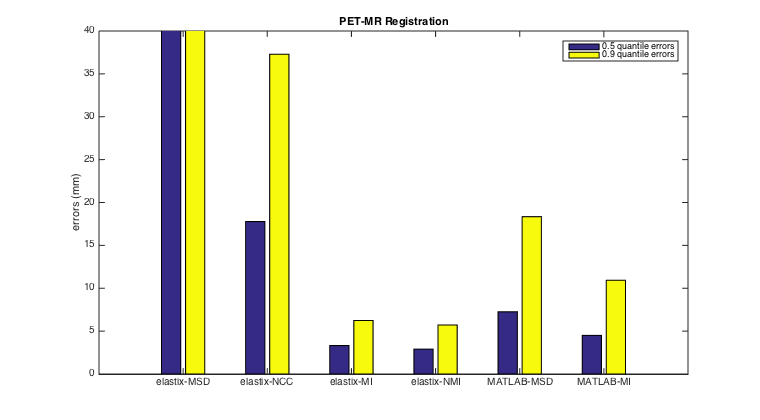
\includegraphics[width=0.5\textwidth]{PET-MR_bars.png}
    \caption{Quantile errors for PET to MR registration. Errors larger than 40 mm have been cut off.}
    \label{fig:PET-MR_bars}
  \end{figure}

  \section{Discussion}

  It can be seen from the figures that implementations using MI or NMI get the best results, both in elastix implementations and MATLAB implementations. NMI seems to perform slightly better than MI. Using MSD for multimodal registration is usually a bad idea, but the results shows that the accuracy MSD implementation using MATLAB is really acceptable, especially when used for PET-MR registration. NCC performs better than MSD, but the errors are still large compared to information theory based approaches.

  \section{Conclusion}

  In this paper, we implement different registration methodologies for 3D/3D rigid registration, including MSD, NCC, MI and NMI based methods, implemented using MATLAB Image Processing Toolbox and/or elastix. Mutual information (MI) and normalized mutual information (NMI) works best, thought NMI is slightly better than MI. The errors of MSD implementations are high, except that the MATLAB version of MSD is capable for PET-MR registration. Normalized correlation coefficient (NCC) performs better than MSD in general, but the errors are still too large compared to MI/NMI approach.

  In conclusion, information theory based approach performs much better than cross-correlation based approach when applied in CT-MR/PET-MR registration.

  \section{Acknowledgment}

  The images and the standard transformation(s) were provided as part of the project, ``Retrospective Image Registration Evaluation'', National Institutes of Health, Project Number 8R01EB002124-03, Principal Investigator, J. Michael Fitzpatrick, Vanderbilt University, Nashville, TN.

  \bibliographystyle{IEEEtran}
  \bibliography{task2}

\end{document}
